\documentclass[11pt, a4paper]{article}
%\usepackage{proj1}
\usepackage{natbib}
\usepackage{fancyhdr}  
\usepackage{subcaption}
\usepackage{caption}
\usepackage{graphicx}
\linespread{1.25} 
\setlength{\parindent}{0cm}
\graphicspath{{Images/}}
\usepackage{hyperref}
\usepackage{amsmath}
\usepackage{amsfonts}
\usepackage{amssymb}
\usepackage{amsthm}
\usepackage{mathtools}
\usepackage{commath}

%\usepackage[sc,osf]{mathpazo}
\usepackage{subcaption}
\usepackage[a4paper, top=1in, left=1.0in, right=1.0in, bottom=1in, includehead, includefoot]{geometry} %Usually have top as 1in

\usepackage{listings}
\usepackage{color} %red, green, blue, yellow, cyan, magenta, black, white
\definecolor{mygreen}{RGB}{28,172,0} % color values Red, Green, Blue
\definecolor{mylilas}{RGB}{170,55,241}


\hypersetup{colorlinks,linkcolor={black},citecolor={blue},urlcolor={black}}
\usepackage{color}
\urlstyle{same}


\theoremstyle{definition}
\newtheorem{definition}{Definition}[section]

\title{Exact Solutions for the Full Problem \\with Force Control and with Flow Control}
\date{}
\newcommand{\Sta}{\rho}
\newcommand{\Adj}{p}
\newcommand{\Con}{u}

\pagenumbering{gobble}
\begin{document}
\lstset{language=Matlab,%
	%basicstyle=\color{red},
	breaklines=true,%
	morekeywords={matlab2tikz},
	keywordstyle=\color{blue},%
	morekeywords=[2]{1}, keywordstyle=[2]{\color{black}},
	identifierstyle=\color{black},%
	stringstyle=\color{mylilas},
	commentstyle=\color{mygreen},%
	showstringspaces=false,%without this there will be a symbol in the places where there is a space
	numbers=left,%
	numberstyle={\tiny \color{black}},% size of the numbers
	numbersep=9pt, % this defines how far the numbers are from the text
	emph=[1]{for,end,break},emphstyle=[1]\color{blue}, %some words to emphasise
	%emph=[2]{word1,word2}, emphstyle=[2]{style},    
    basicstyle=\footnotesize\ttfamily,
}

\section*{Report on weekly progress; meeting 02/04/2020}
\subsection*{Perturbation Functions Considered}
The one from last week:
\begin{align*}
f(t) = \frac{e^{-1/t}}{e^{-1/t} + e^{-1/(1-t)}}.
\end{align*}
An new perturbation is given by:
\begin{align*}
g(t) = \frac{e^{-a/(t-t0)}}{e^{-a/(t-t0)}+ e^{-a/(1-t-t0)}} \times \frac{e^{a/(t-t0)}}{e^{a/(t-t0)}+ e^{a/(1-t-t0)}},
\end{align*}
where $a=0.7$ (mostly) and $t0 = -0.01$. The translation by $t0$ is due to the fact that otherwise you'd get NANs for $t=0$. The factor $a$ is flattening or sharpening the peak. While $g(t)$ is perturbed up to $0.04$ (see Figure 1, perturbation in time), this does not translate to the perturbation in $w$. For a perturbation in $w$ of $0.1$, you need $0.05g(t)$ (see Figure 1 for perturbation $0.1g(t)$).
\begin{figure}[h]
	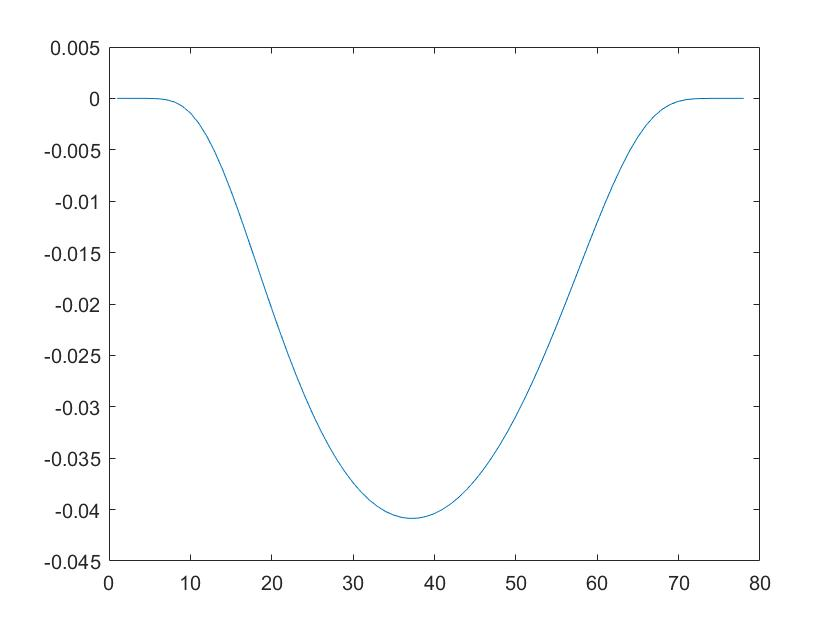
\includegraphics[scale=0.3]{Pertfun1.jpg}
	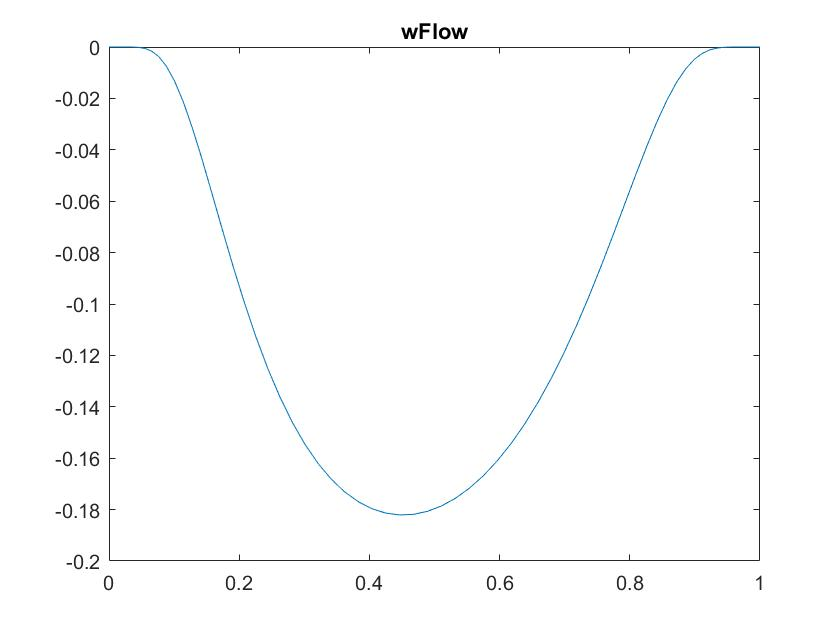
\includegraphics[scale=0.3]{Pertw1.jpg}
	\caption{Perturbation $g(t)$ (left), $w$ perturbed by $0.1g(t)$ (right).}
\end{figure}

\subsection*{Kalise Algorithm}
\subsubsection*{Exact Solution Errors}
I have noticed that when measuring the error in the L2Linfinity sense (as done in the past weeks), this algorithm shows a difference of up to 2 orders of magnitude between $w,p$ and $\rho$. The most severe case is the mixed BC one, where the difference can go up to 4 orders of magnitude (depending on $\beta$ - smaller $\beta$ increase the error).
This seems to be mitigated by measuring the error pointwise. Furthermore, distributing $\beta$ in the exact solutions between $\rho$ and $p$ instead of just putting it on $p$, seems to improve the situation in the mixed boundary condition case.
This has not shown to be a problem in the Multiple Shooting algorithm.
Using the exact solution that is linear in time for the Mixed BCs (see other document) solves the problem in the L2Linf norm as well. The algorithm error is much less than the ODE tolerance for all variables.
This pattern is also not there for Dirichlet/Neumann solutions with linear time (i.e. trig in space, linear in time).

\subsubsection*{Neumann Flow Control (plus2) $\beta = 10^{-3}$}
Further to last week, I have tested Neumann (plus 2) flow control with $\beta = 10^{-3}$. This converges in $7210$ Iterations with $\lambda = 1$, tolerances = $10^{-9}/10^{-5}$ and $n=74$, $N=72$. The perturbation used is $0.1f(t)$, as before. The consistency error is $w = 9.9920 \times 10^{-6}$ and the exact errors are $w_{err}= 9.4017 \times 10^{-6}$, $p_{err} = 5.8640 \times 10^{-5}$ and $\rho_{err} = 8.0369 \times 10^{-6}$, see Figure 2.
\begin{figure}[h]
	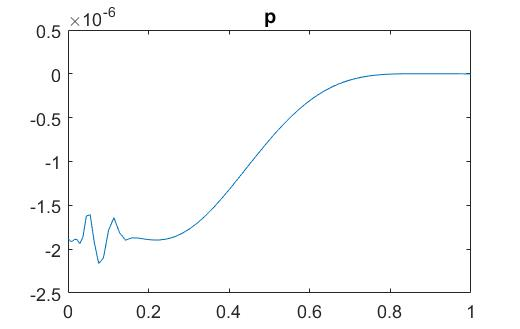
\includegraphics[scale=0.3]{KalNp1.jpg}
	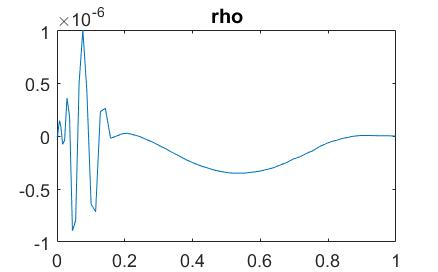
\includegraphics[scale=0.3]{KalNrho1.jpg}
	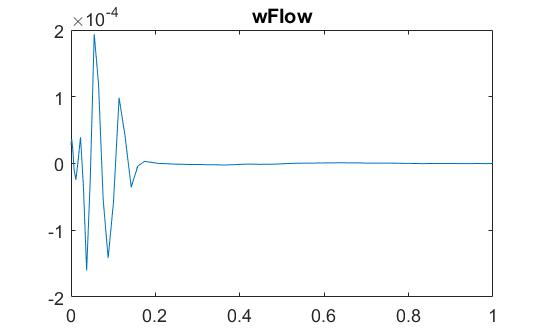
\includegraphics[scale=0.3]{KalNw1.jpg}
	\caption{Exact Errors, Neumann Flow Control $\beta = 10^{-3}$, perturbation $0.1f(t)$.}
\end{figure}
\subsubsection*{Mixed Boundary Conditions}
Using 'ADFlowMixedExact' as exact solution (see exact solution for mixed BCs). Here, $\beta =10^{-1}$, tolerances are $10^{-9}/10^{-5}$, $\lambda =0.01$, $n=74$, $N=72$. The perturbation is again $0.1f(t)$.
This converges in $7463$ Iterations, consistency error is $9.9958 \times 10^{-6}$, exact errors are $w_{err} = 2.4073 \times 10^{-5}$, $p_{err} = 2.4526 \times 10^{-5}$ and $\rho_{err} = 7.4239 \times 10^{-7}$, see Figure 2.
Note that the errors are two orders of magnitude apart in the chosen norm, however not on the figure. Compare with exact solution above.
\begin{figure}[h]
	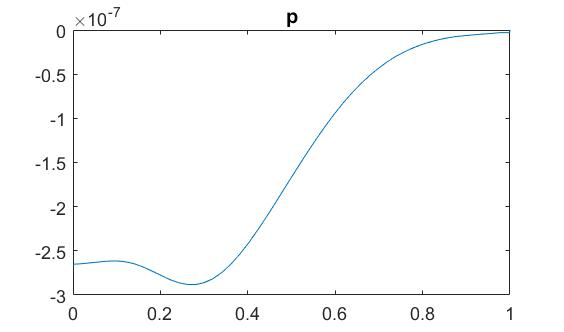
\includegraphics[scale=0.3]{KalMp1.jpg}
	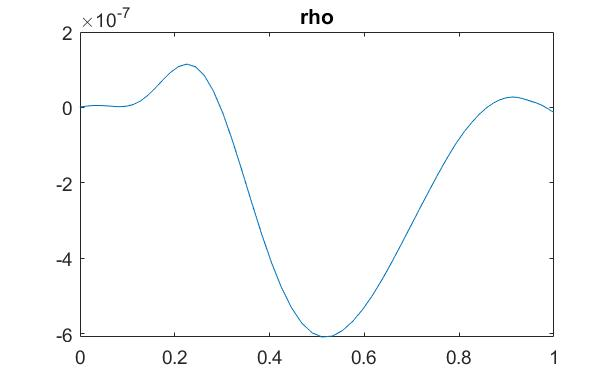
\includegraphics[scale=0.2]{KalMrho1.jpg}
	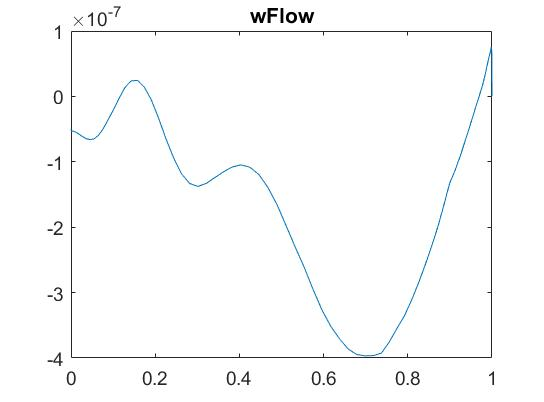
\includegraphics[scale=0.3]{KalMw1.jpg}
	\caption{Exact Errors, Neumann Flow Control $\beta = 10^{-3}$, perturbation $0.1f(t)$.}
\end{figure}
\subsubsection*{Investigating Pointwise Error for Kalise}
Investigating Neumann (plus2) Flow Control shows that for $\beta = 10^{-1}$ with $\lambda =0.01$ and $0.005$, the result diverges after a while. The relative error in $p$ is $7.49...$. Trying $\beta = 10^{-3}$ diverges after three iterations when trying $\lambda = 1, 0.5, 0.01$. Given that this converges in the L2Linfty norms, it doesn't seem like pointwise error is good for the convergence of the Kalise method. (However, it does fix the odd behaviour in exact solution - see above.)\\
Doing the same thing for Dirichlet flow with $\beta =10^{-1}$ and $\lambda =0.01$, it diverges at a consistency of $3.4502 \times 10^{-4}$ at Iteration $2776$. 
This is using the perturbation $0.1f(t)$, with tolerances $10^{-9}/10^{-5}$ and $n=74$, $N=72$. Same happens with $10^{-12}$. When giving the diverged result to the multiple shooting algorithm, it diverges further, so that's not a solution.

\subsection*{Checking that Multiple Shooting converges given the Kalise solution}
Using the Kalise result for the Neumann Flow Control Problem with $\beta =10^{-1}$ and giving this to the multiple shooting algorithm as an initial guess for $\rho$ and $p$. The Kalise algorithm converges in $7209$ Iterations (compare with above), with $\lambda =0.01$, tolerances = $10^{-12} / 10^{-5}$, $n=74$, $N = 72$. The consistency error is $w = 9.9992 \times 10^{-6}$.
Then the multiple shooting, with $\lambda = 0.1$, has an initial consistency error of $0.00001058$, with exact errors $\rho_{err} = 0.00000802$ and $p_{err} = 0.00005765$. This converges in $20$ Iterations to a consistency of $0.00000997$, with exact errors $\rho_{err} = 0.00000821$ and $p_{err} = 0.00005745$. So the exact error in $\rho$ diverges, while the one in $p$ converges. Overall, the Kalise solution is a solution to the multiple shooting algorithm as well.


\subsection*{Multiple Shooting}
\subsubsection*{Using Kalise as initial guess, then Multiple shooting}
This is doing one Kalise step first to get an initial guess for $p$ (instead of integrating). In the pointwise norm the error in $p$ is $7.49588...$ and in $\rho$  $0.3589...$. This eventually diverges and the error is as erratic as we saw last week. This is Neumann (plus2) Flow Control, $\beta = 10^{-1}$ and perturbation $0.1 f(t)$.
\subsubsection*{Multiple Shooting with Integration and PW error}
Using the same technique as last week by getting an initial guess for $p$ from integrating the gradient equation. This also converges for a while before diverging, as last week.
This is Neumann (plus2) Flow Control, $\beta = 10^{-1}$ and perturbation $0.1 f(t)$.



\subsection*{Different Perturbations}
Using the different perturbations introduced above (in very first section).

\subsubsection*{Kalise Algorithm}
Using L2Linf norm (since PW doesn't seem to converge), tols $= 10^{-9}/10^{-5}$, $n=74$, $N=72$. Considering Neumann (plus2) flow control and a perturbation of $0.1g(t)$. For $\beta = 10^{-1}$ and $\lambda = 0.01$, it converges. 
It needs a bit more than $5000$ Iterations and the exact errors are $w_{err}= 1.4136 \times 10^{-5}$, $p_{err} = 7.7223 \times 10^{-5}$ and $\rho_{err}= 1.3989 \times 10^{-5}$ (see Figure \ref{FigKal1}). So here, to get $10^{-5}$ accuracy, the consistency tolerance would have to be lower. When investigating this, we set the consistency tolerance to $10^{-6}$ and leave everything else the same. The algorithm diverges at $w=5.1200 \times 10^{-6}$, with exact errors of $w_{err}= 1.8839 \times 10^{-5}$, $p_{err}=4.5021 \times 10^{-5}$ and $\rho_{err}=1.8175 \times 10^{-5}$. This shows that we cannot get to an error of $O(10^{-5})$ with these configurations.\\
\begin{figure}[h]
	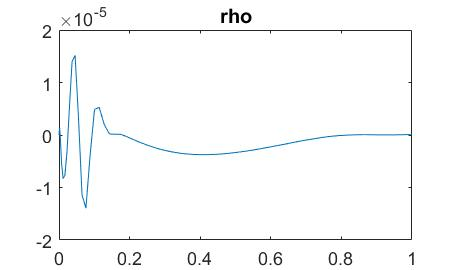
\includegraphics[scale=0.3]{KalCreatewFlow7L2Linf1.jpg}
	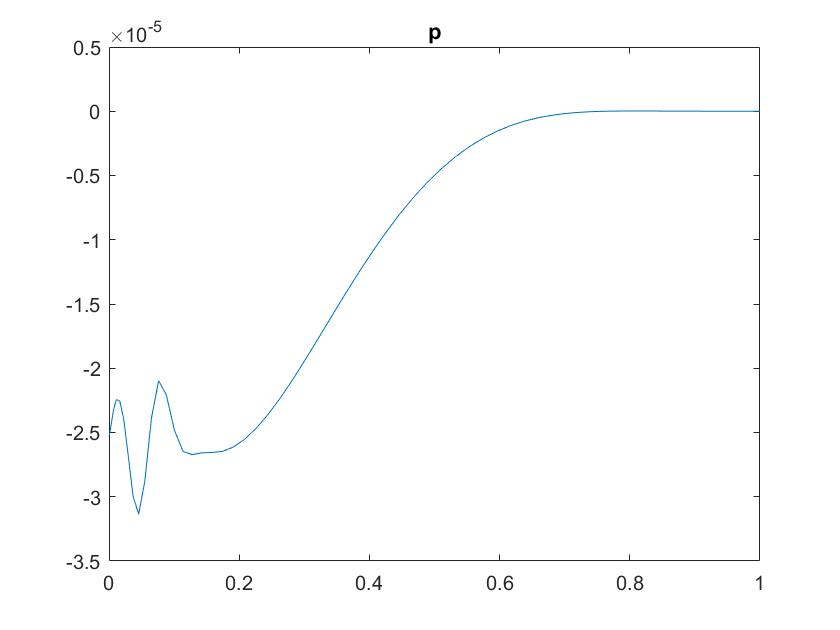
\includegraphics[scale=0.2]{KalCreatewFlow7L2Linf2.jpg}
	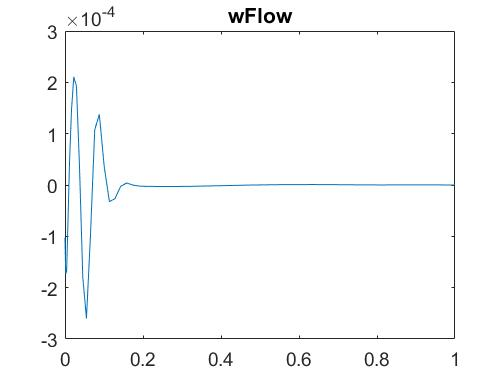
\includegraphics[scale=0.25]{KalCreatewFlow7L2Linf3.jpg}
	\caption{Exact Errors, Neumann Flow Control $\beta = 10^{-1}$, perturbation $0.1g(t)$.}
	\label{FigKal1}
\end{figure}
The next thing to try is $\beta = 10^{-3}$ and $\lambda =1$. This also converges in $5980$ Iterations. Then the exact errors are $w_{err}=1.6386 \times 10^{-5}$, $p_{err}=7.7389 \times 10^{-5}$ and $\rho_{err} = 1.5156 \times 10^{-5}$. This is very similar to the case when $\beta =10^{-3}$.\\
Now it should be investigated how $0.05g(t)$ converges, considering that this is a $10\%$ perturbation in $w$.\\


Dirichlet Flow control is not working as well as Neumann. Using the L2Linf errors, $\beta =10^{-1}$, tols $=10^{-9}/10^{-5}$ and $\lambda =0.01$. When perturbing by $0.1 g(t)$, the algorithm diverges after $1864$ Iterations at a consistency of $2.4847 \times 10^{-4}$. The exact errors at that point are  $w_{err} = 4.2662 \times 10^{-4}$, $p_{err}= 2.4504 \times 10^{-4}$ and $\rho_{err} = 3.5706 \times 10^{-4}$, see Figure \ref{FigKal2}. Measuring the pointwise error of this result is worse. 
When choosing $0.01g(t)$, the algorithm diverges at $w=2.4800 \times 10^{-5}$ and when choosing $0.01g(t)$ with $a=0.5$ it diverges at $5.3647 \times 10^{-5}$ at Iteration $1524$. When taking the result and translating it to pointwise errors we get $w_{err} = 5.1272 \times 10^{-4}$, $p_{err}=1.1953 \times 10^{-4}$ and $\rho_{err}= 2.6470 \times 10^{-4}$.
When using pointwise error as the convergence measure from the start for this problem, it diverges at $w= 2.8653 \times 10^{-4}$ with exact errors of $w_{err}=5.3481 \times 10^{-4}$, $p_{err}=1.2412 \times 10^{-4}$ and $\rho_{err}=2.8613$. This shows that using the pointwise error for this problem, the convergence is slightly worse than if we use L2Linf error. There is no apparent reason for this to not converge since the perturbation in $w$ is small, see Figure \ref{FigKal3}.
\begin{figure}[h]
	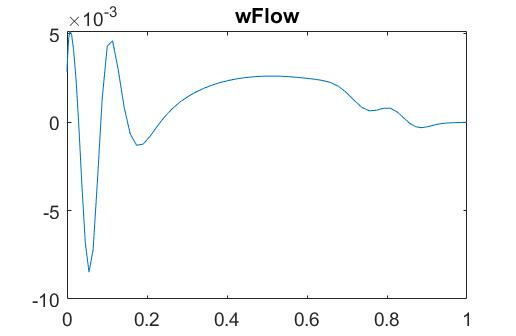
\includegraphics[scale=0.3]{KalD1.jpg}
	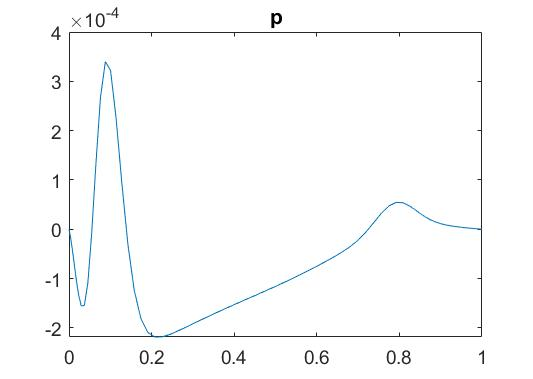
\includegraphics[scale=0.2]{KalD2.jpg}
	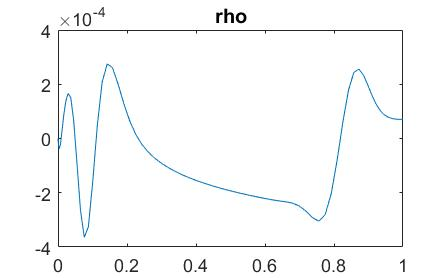
\includegraphics[scale=0.25]{KalD3.jpg}
	\caption{Exact Errors, Dirichlet Flow Control $\beta = 10^{-1}$, perturbation $0.1g(t)$.}
	\label{FigKal2}
\end{figure}

\begin{figure}[h]
	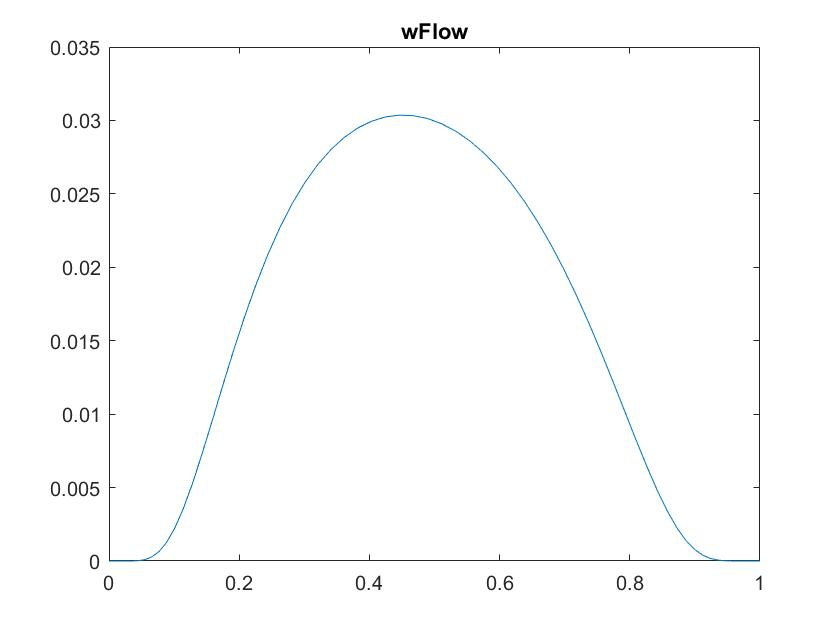
\includegraphics[scale=0.25]{wpert1.jpg}
	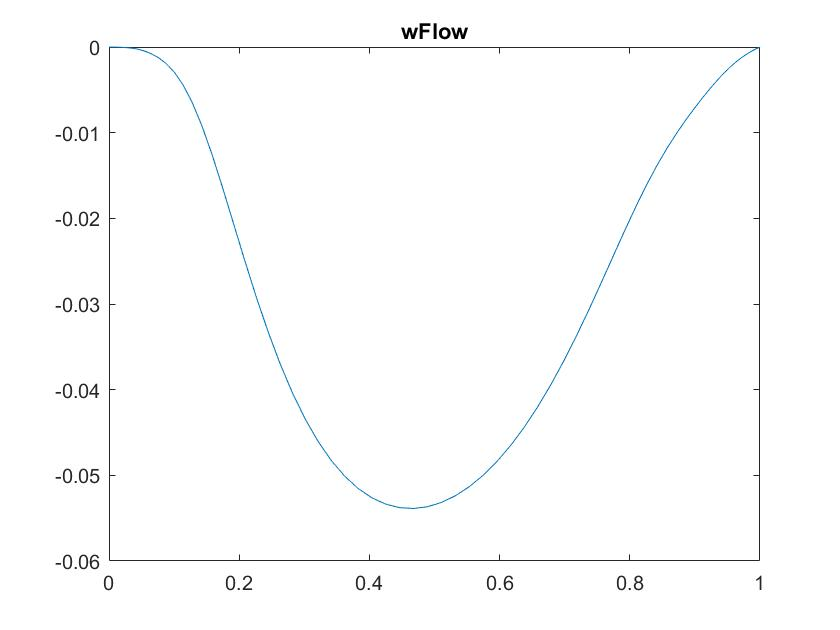
\includegraphics[scale=0.25]{wpert2.jpg}
	\caption{Perturbation in $w$ (first and second vs exact solution), perturbation $0.01g(t)$, $a=0.5$.}
	\label{FigKal3}
\end{figure}



Mixed Boundary conditions with a linear time relationship (see document for exact solution).
\subsubsection*{Multiple Shooting}
Using Neumann (plus2) and Flow control at first we try $0.1g(t)$ as perturbation, with again $N=72$, $n=74$, tols$=10^{-9}/10^{-5}$, $\beta= 10^{-1}$ and $\lambda =0.1$. 
Using the pointwise error measure, this converges to a consistency of $0.00514602$ at Iteration $214$, while $\rho_{err} = 0.00011263$ at Iteration $211$ and $p_{err}=0.06646699$ at Iteration $247$ are the lowest individual exact errors. This is from an initial error of $0.05973065$ with exact errors of $\rho_{errI} = 0.06184073$ and $p_{errI} = 0.02023870$. The initial guess for $p$ is found by integrating the gradient equation. Finding the initial guess for $p$ using the Kalise algorithm makes it worse and it converges only to $0.03...$ consistency.
Using the L2Linfinity error with a change in the perturbation $0.1g(t)$ with $a=0.5$ instead (Doesn't significantly change errors in pointwise measure, makes it slightly worse), it gives better results.
It converges to $0.00043827$ at Iteration $218$ and with $\rho_{err} = 0.00009809$ at Iteration $202$ and $p_{err}= 0.00445544$ at Iteration $245$. So at least this example suggests that the L2Linf error is a better fit.
Investigating the possible perturbations that might converge, the next choice is $0.01g(t)$ and $a=0.5$ with L2Linf norm. The initial error is $0.00282653$ with $\rho_{errI}= 0.00198820$ and $p_{errI}=0.00045162$ ($p$ diverges before converging). This diverges at $0.00004813$ at Iteration $196$ with $\rho_{err} = 0.00001212$ and $p_{err} = 0.00048389$ at Iteration $197$ with $p$ converging further after that, see Figure \ref{FigMult1} and \ref{FigMult2}. 
Next, try to decrease $\lambda$ to see if it improves convergence.It actually makes the convergence slightly worse $0.000049...$ and takes a lot longer. 
\begin{figure}[h]
	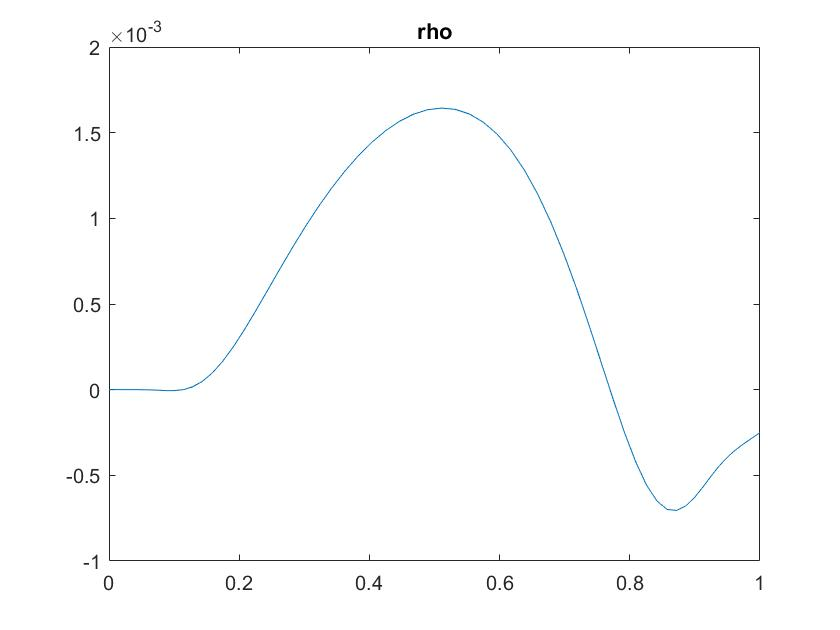
\includegraphics[scale=0.2]{MultN1.jpg}
	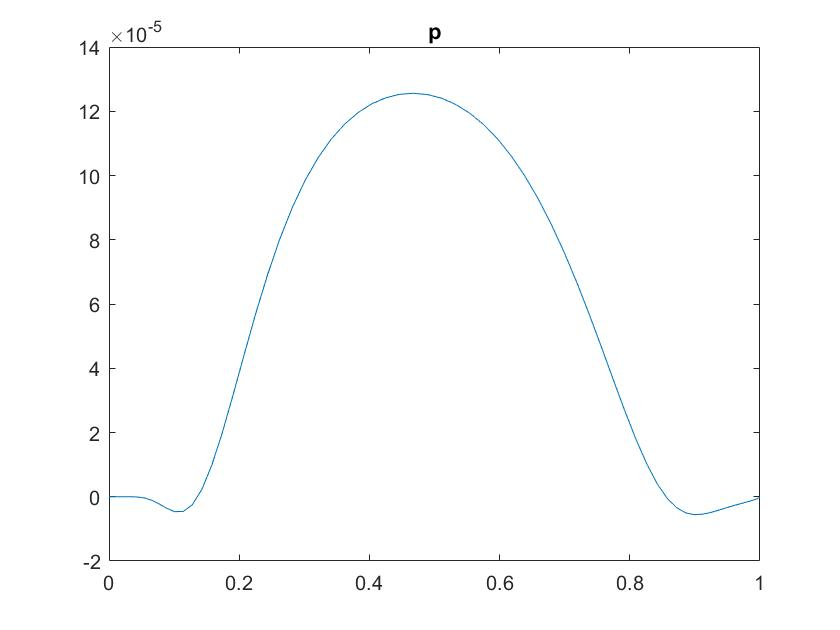
\includegraphics[scale=0.2]{MultN2.jpg}
	\caption{Initial Exact Errors, Neumann Flow Control $\beta = 10^{-1}$, perturbation $0.01g(t)$, $a=0.5$.}
	\label{FigMult1}
\end{figure}
\begin{figure}[h]
	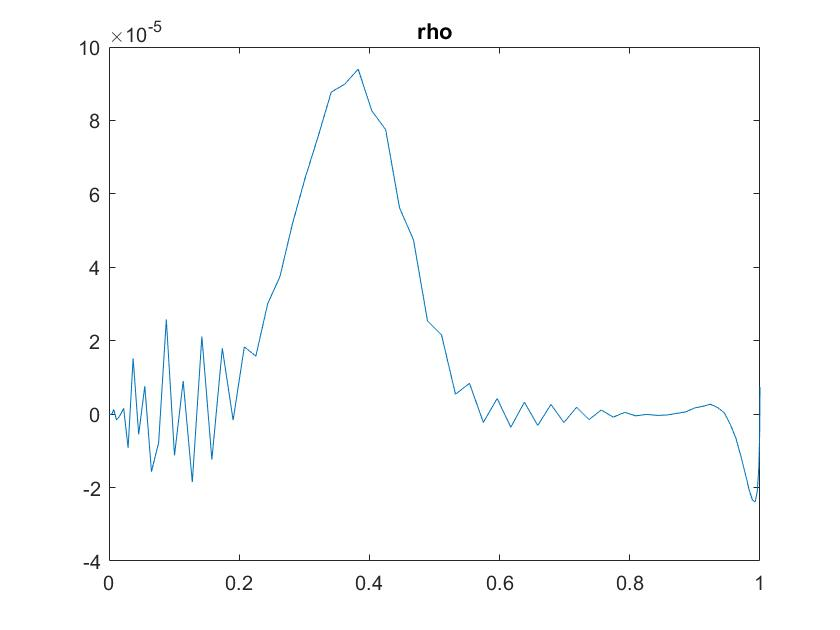
\includegraphics[scale=0.2]{MultNfin1.jpg}
	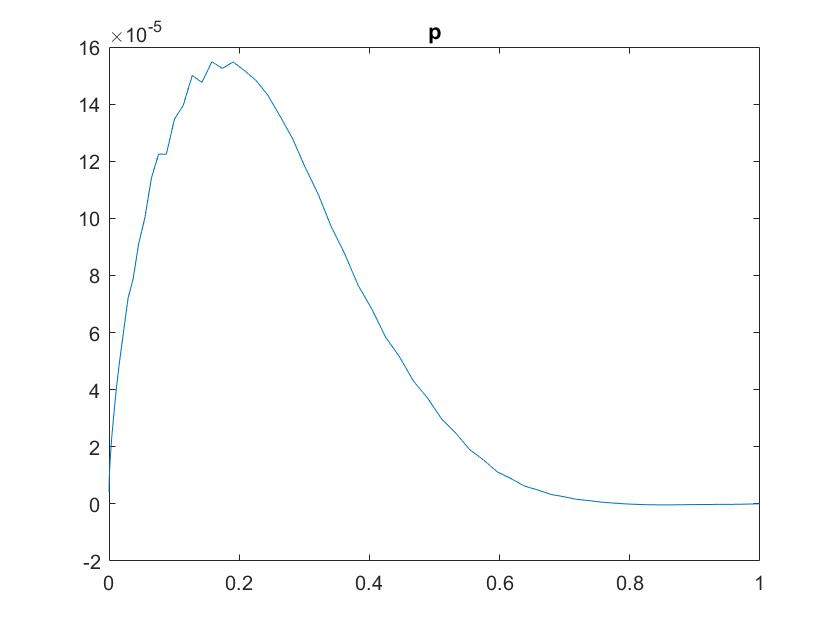
\includegraphics[scale=0.2]{MultNfin2.jpg}
	\caption{Exact Errors, Neumann Flow Control $\beta = 10^{-1}$, perturbation $0.01g(t)$, $a=0.5$.}
	\label{FigMult2}
\end{figure}

\subsection*{Linear time exact solution trials}
\subsubsection*{Kalise}
We are using the exact solution 'Mixed3' with Dirichlet and Neumann BCs. All errors are measured in L2Linf, tolerances and $n,N$ as above.
In the Dirichlet Case both $\beta = 10^{-1}$ ($\lambda =0.1$) and $\beta = 10^{-3}$ ($\lambda =10$) converged. The perturbation was $10g(t)$ with $a=0.7$, see Figure \ref{Figlint1} and \ref{Figlint2}.
For $\beta=10^{-1}$ the initial exact error was $w_{errI}= 0.0324$, $p_{errI} = 0.0557$ and $\rho_{errI}= 0.0421$. Then after $1157$ iterations it converged to $w_{err}= 2.2602 \times  10^{-7}$, $p_{err} = 4.2460 \times 10^{-7}$ and $\rho_{err} = 31175 \times 10^{-7}$. The errors for $\beta = 10^{-3}$ are similar.\\
The results for the Neumann case are very similar. The algorithm converges for both $\beta$ values. 
For $\beta = 10^{-1}$ the initial exact errors are $w_{ErrI}=0.0309$, $p_{errI} = 0.0755$ and $\rho_{ErrI}= 0.0466$. Then in $1175$ Iterations, this converges to $w_{err}= 2.1936 \times 10^{-7}$, $p_{Err}=6.5744 \times 10^{-7}$ and $\rho_{err} = 3.4265 \times 10^{-7}$. The results for $\beta = 10^{-3}$ are again similar.\\
\begin{figure}[h]
	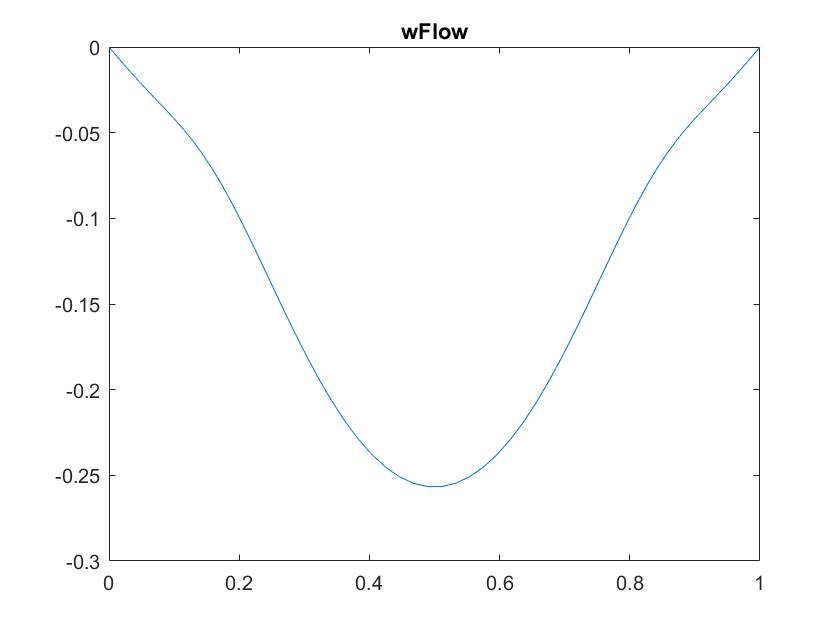
\includegraphics[scale=0.3]{wFlint3.jpg}
	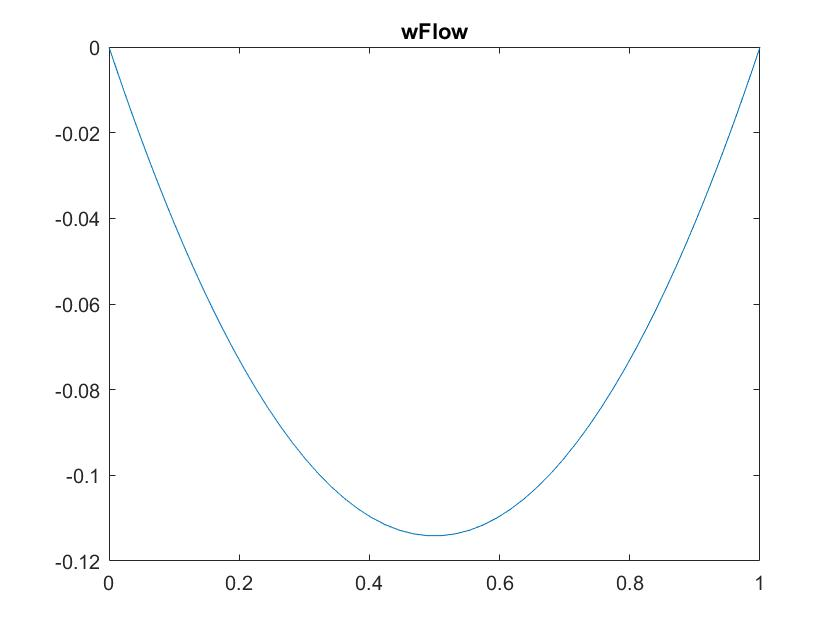
\includegraphics[scale=0.3]{wFlint4.jpg}
	\caption{Perturbed $w$ and exact $w$.}
	\label{Figlint1}
\end{figure}
\begin{figure}[h]
	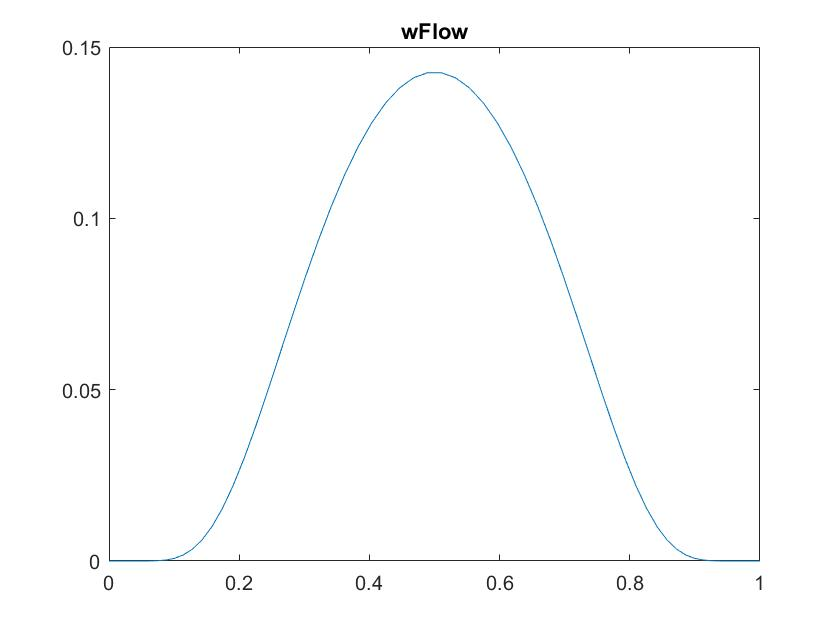
\includegraphics[scale=0.2]{wFlint1.jpg}
	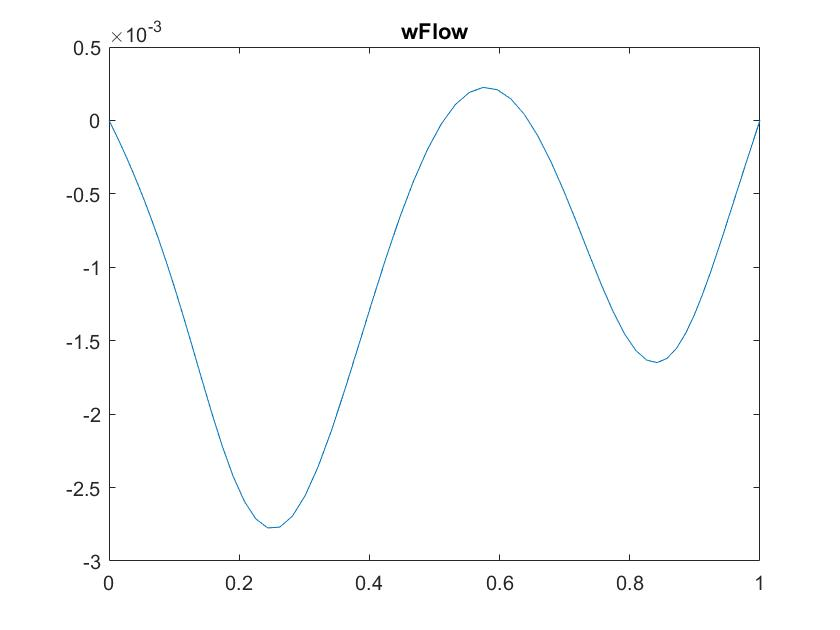
\includegraphics[scale=0.2]{wFlint2.jpg}
	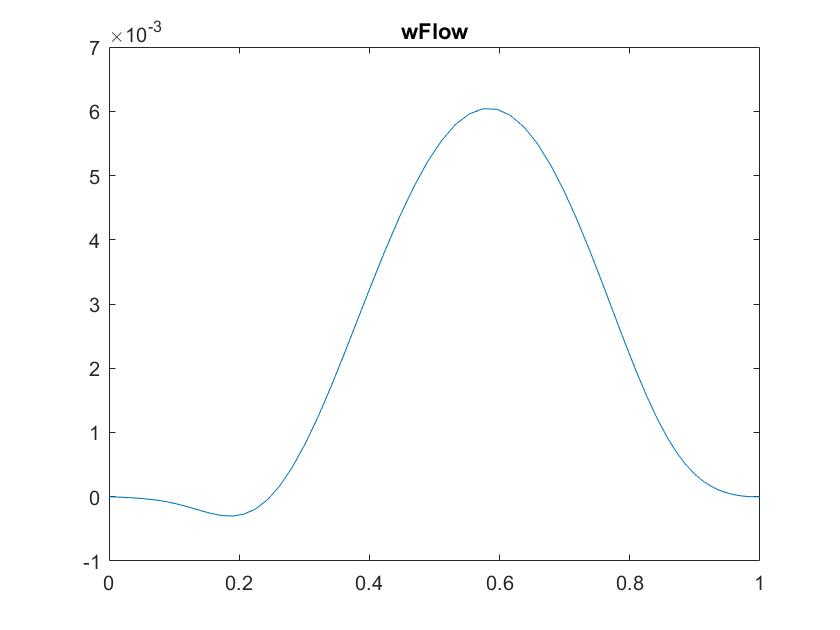
\includegraphics[scale=0.2]{wFlint5.jpg}
	\caption{Perturbed $w$ Error (first - left) (second: Dirichlet - Mid, Neumann - right).}
	\label{Figlint2}
\end{figure}

Now, investigating Neumann (plus 2) with linear time terms (i.e. exact solution with trig functions in space, and linear time) gives the following: With $\beta=10^{-1}$ the initial errors are $w_{errI} = 0.2353$, $p_{errI} = 0.8576$ and $\rho_{errI}=0.3192$. This converges in $1167$ Iterations to $w_{err}=6.9449 \times 10^{-7}$, $p_{err}= 8.3209 \times 10^{-6}$ and $\rho_{err}= 2.1389 \times 10^{-6}$. The results are very similar for $\beta=10^{-3}$ and can be seen in Figure \ref{Figlint3}. The perturbation in $w$ can be seen in Figure \ref{Figlint3a}. Note this also converges to  a tolerance of $10^{-6}$ instead of $10^{-5}$.\\
\begin{figure}[h]
	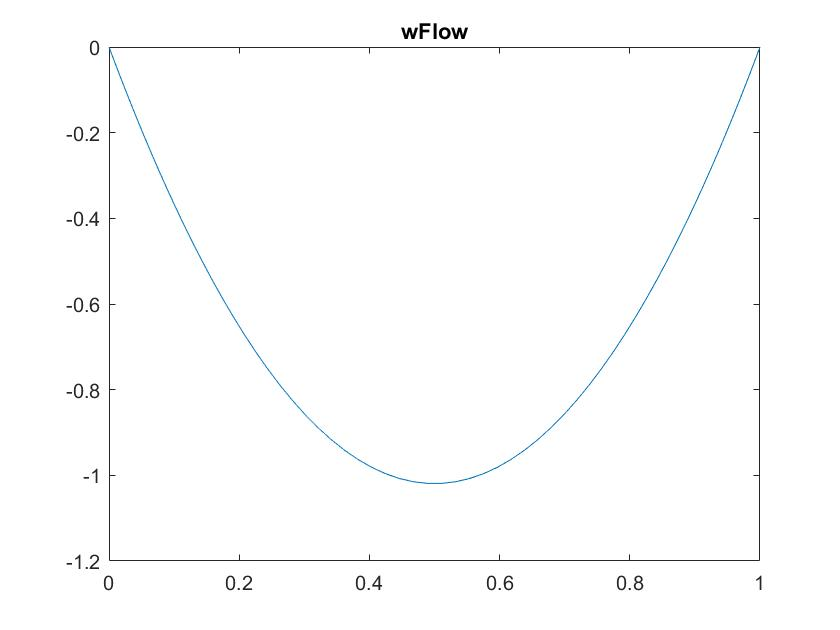
\includegraphics[scale=0.3]{linNwexact1.jpg}
	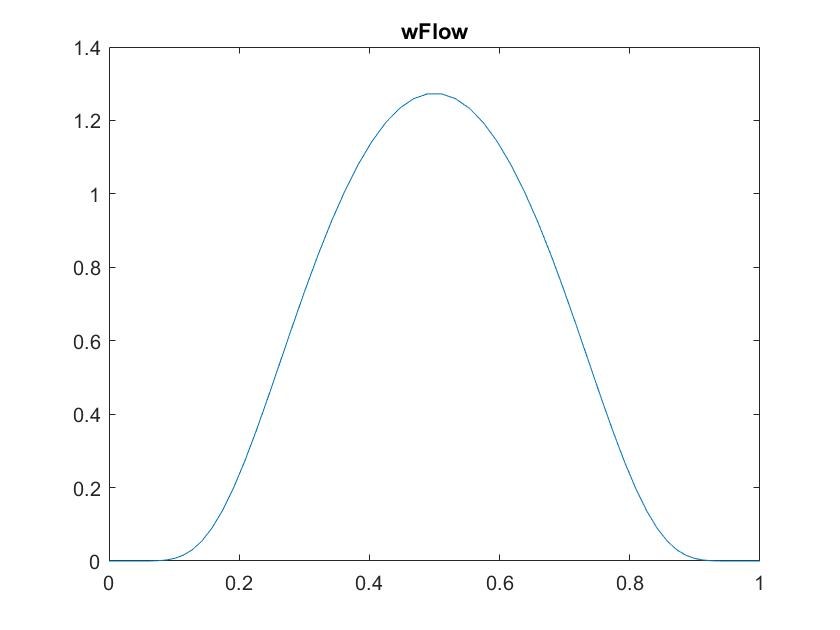
\includegraphics[scale=0.3]{linNwerr1.jpg}
	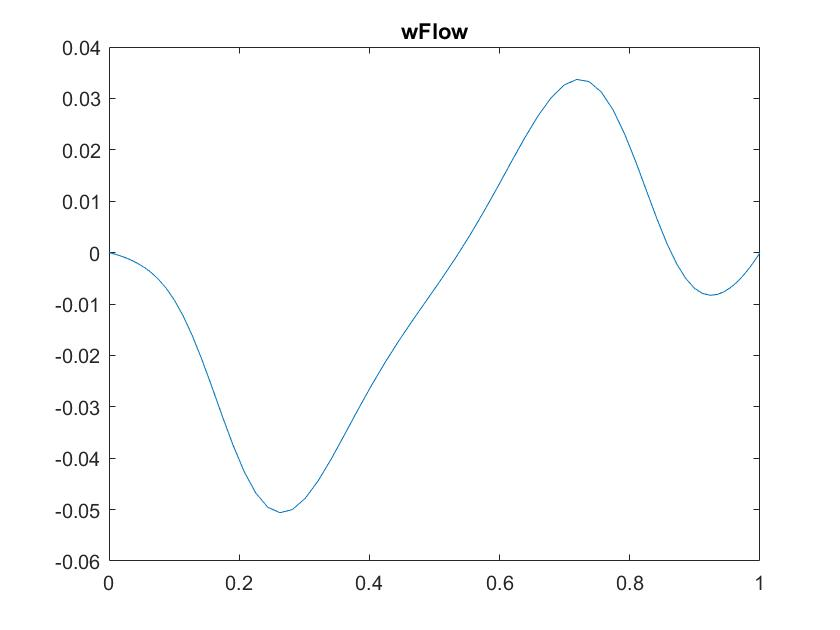
\includegraphics[scale=0.3]{linNwerr2.jpg}
	\caption{This is $w$ exact (left), $w$ first error (mid) and second error (right). Here with $\beta =10^{-3}$ and perturbation $10g(t)$.}
	\label{Figlint3a}
\end{figure}

\begin{figure}[h]
	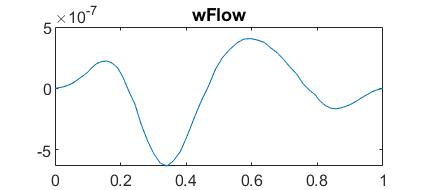
\includegraphics[scale=0.35]{linNfin1.jpg}
	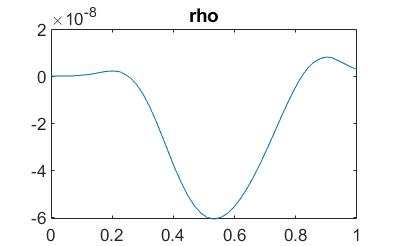
\includegraphics[scale=0.35]{linNfin2.jpg}
	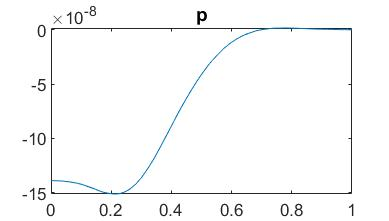
\includegraphics[scale=0.35]{linNfin3.jpg}
	\caption{Final error in variables when Neumann with linear time converged. Here with $\beta =10^{-3}$ and perturbation $10g(t)$.}
	\label{Figlint3}
\end{figure}

Looking at Dirichlet Exact solutions with linear time terms (i.e. trig in space, linear in time), this also converges for the two $\beta$ values. Accidentally the tolerance was set to $10^{-6}$ which converged as well ($\beta = 10^{-1}$. The perturbations in $w$ can be seen in Figure \ref{Figlint4a}.
The results are $w_{err} = 8.6507 \times 10^{-7}$, $p_{err} = 2.9450 \times 10^{-7}$ and $\rho_{Err}= 10^{-7}$. \\
Considering $\beta+10^{-3}$ seems to be a bit more difficult, simply because the scaling makes the perturbation much larger for this case. Therefore, different perturbations have to be tried, to see which one perturbs $w$ a reasonable amount. This is most likely due to the fact that the Dirichlet exact solution for $w$ scales like $1/\beta$ (to be consistent with the original exact solutions). This should be checked.
\begin{figure}[h]
	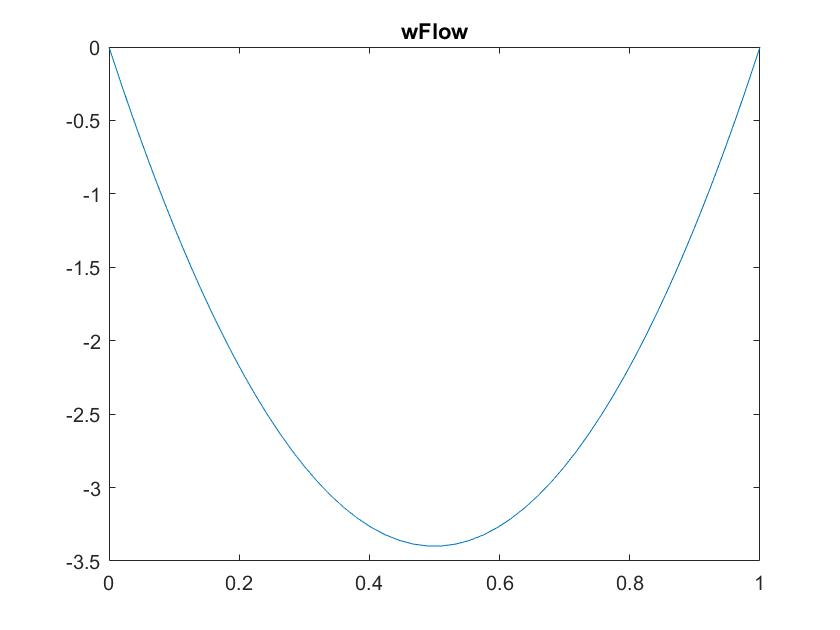
\includegraphics[scale=0.3]{linDwexact1.jpg}
	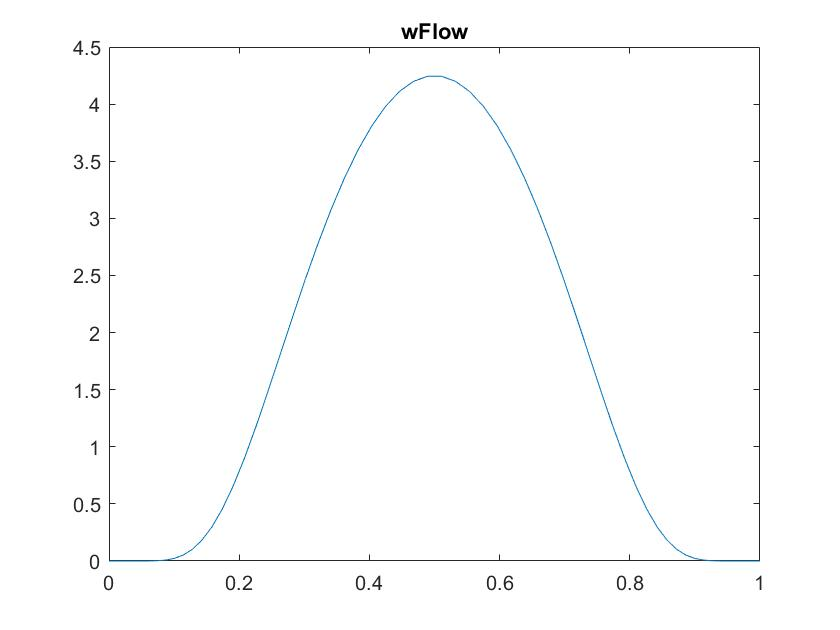
\includegraphics[scale=0.3]{linDwerr1.jpg}
	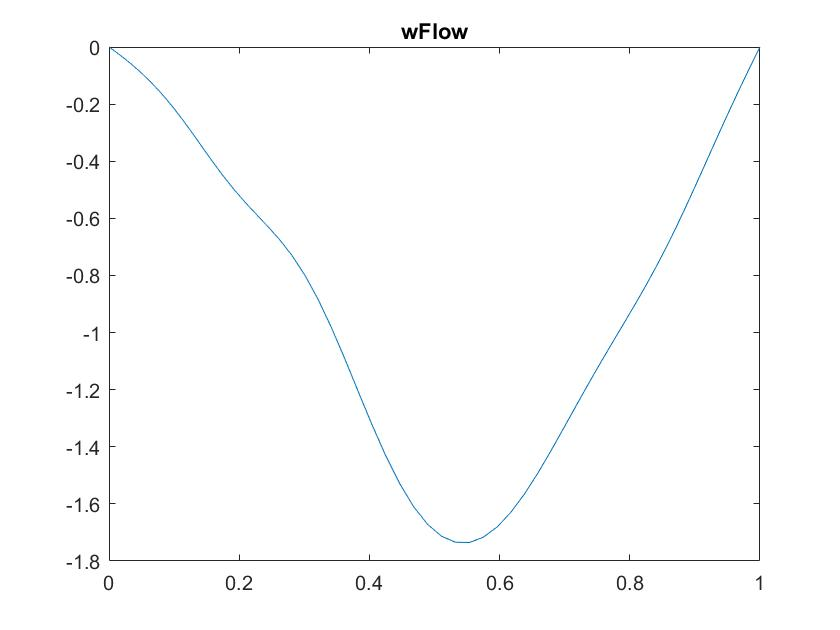
\includegraphics[scale=0.3]{linDwerr2.jpg}
	\caption{This is $w$ exact (left), $w$ first error (mid) and second error (right). Here with $\beta =10^{-1}$ and perturbation $10g(t)$.}
	\label{Figlint4a}
\end{figure}

\subsubsection*{Multiple Shooting}
Using 'Mixed3' again, and the perturbation $10g(t)$,with $\beta=10^{-1}$ and measured in L2Linf norm, Multiple Shooting converges within $724$ Iterations. The exact errors are then $\rho_{err} = 0.00000791$ and $p_{err}=0.00015429$, see Figure \ref{Figlint5}. The initial errors were $cons_{err} = 0.02820414$, $\rho_{ErrI} = 0.03215880$ and $p_{err} = 0.01302147$. 

\begin{figure}[h]
	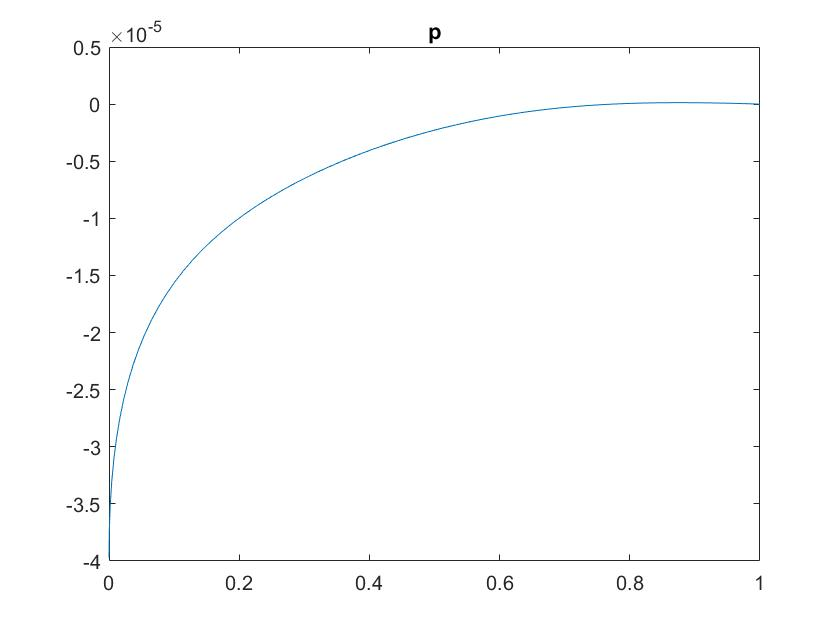
\includegraphics[scale=0.3]{MultMD1.jpg}
	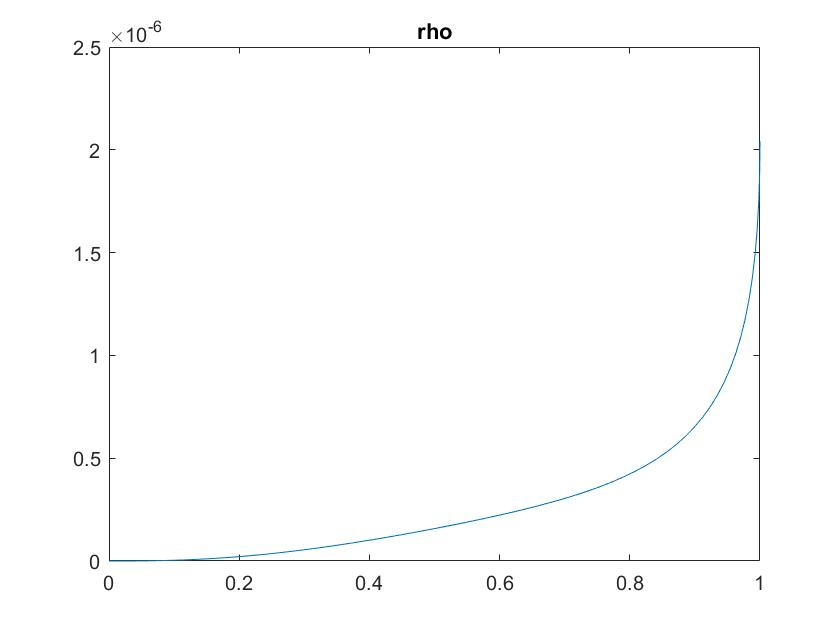
\includegraphics[scale=0.3]{MultMD2.jpg}
	\caption{Final exact error in $\rho$ and $p$. Here with $\beta =10^{-1}$ and perturbation $10g(t)$.}
	\label{Figlint5}
\end{figure}
\end{document}